\documentclass[twocolumn,aps,prd,superscriptaddress]{revtex4-1}  
\usepackage{amsmath,graphicx}

\DeclareMathOperator{\Tr}{Tr}

\usepackage{natbib}
\usepackage{amsmath,amssymb}

\usepackage[usenames]{color}
\newcommand{\CiteNeed}{\textcolor{red}{\scriptsize[citation needed]}}
\newcommand{\sv}[1]{\textcolor{blue}{\it{\textbf{sv: #1}}} }
\newcommand{\ki}[1]{\textcolor{cyan}{\it{\textbf{ki: #1}}} }

\newcommand{\Agw}{\ensuremath{A_\mathrm{gw}}}
\newcommand{\res}{\ensuremath{\delta {\bf t}}}

\begin{document}

\title{Assessing spatial correlations in pulsar timing arrays with the noise-marginalized optimal statistic}


\author{Sarah J.\ Vigeland}
\affiliation{Center for Gravitation, Cosmology and Astrophysics, University of Wisconsin--Milwaukee, PO Box 413, Milwaukee WI, 53201, USA}

\author{Kristina P.\ Islo}
\affiliation{Center for Gravitation, Cosmology and Astrophysics, University of Wisconsin--Milwaukee, PO Box 413, Milwaukee WI, 53201, USA}

\author{Stephen R.\ Taylor}
\affiliation{Jet Propulsion Laboratory, California Institute of Technology, 4800 Oak Grove Drive, Pasadena, California 91106, USA}
\affiliation{Theoretical AstroPhysics Including Relativity (TAPIR), MC 350-17, California Institute of Technology, Pasadena, California 91125, USA}

\author{Justin A.\ Ellis}
\affiliation{Department of Physics and Astronomy, West Virginia University, P.O. Box 6315, Morgantown, WV 26506, USA}
\affiliation{Center for Gravitational Waves and Cosmology, West Virginia University, Chestnut Ridge Research Building, Morgantown, WV 26505, USA}

\author{Xavier Siemens}
\affiliation{Center for Gravitation, Cosmology and Astrophysics, University of Wisconsin--Milwaukee, PO Box 413, Milwaukee WI, 53201, USA}

\date{\today}  

\begin{abstract}
Observations have revealed that nearly all galaxies contain supermassive black holes (SMBHs) at their centers, 
with masses between \sv{look up}. 
When galaxies merge, these SMBHs form SMBH binaries (SMBHBs), 
which emit low-frequency gravitational waves (GWs). 
The incoherent superposition of these GW sources produce a stochastic GW background (GWB) 
that can be observed by pulsar timing arrays (PTAs). 
The optimal statistic is a frequentist estimator for the amplitude of a GWB 
that specifically looks for the spatial correlations induced by the GWB in PTA data. 
In this paper, we introduce an improved method for computing the optimal statistic 
that marginalizes over the red noise in individual pulsars. 
We use simulations to demonstrate that this method 
more accurately determines the strength of a GWB, 
and we use the noise-marginalized optimal statistic to assess the 
significance of different spatial correlations and 
by performing sky scrambles.
\end{abstract}

\maketitle


\section{Introduction}

Long-wavelength gravitational waves (GWs) with frequencies of 
$10^{-9} - 10^{-7} \; \mathrm{Hz}$ can be observed with pulsar timing arrays (PTAs) 
composed of millisecond pulsars (MSPs) \cite{hd1983,fb1990}. 
The dominant astrophysical source in this frequency range is an isotropic stochastic 
gravitational wave background (GWB) 
made up of the incoherent superposition of GWs from inspiraling 
supermassive black hole binaries (SMBHBs) 
\citep{1995ApJ...446..543R, 2003ApJ...583..616J, 2003ApJ...590..691W}. 
By monitoring the ultra-regular periodic emission from these pulsars using radio telescopes, 
we can probe the dynamics of the spacetime through which the pulses travel. 
This is done by searching for correlations in the pulsar timing residuals, 
which measure the difference between the expected and observed pulse times of arrival. 
Current upper-limits on the stochastic background from PTAs are approaching 
theoretical predictions for the stochastic GWB \citep{PPTA2013,EPTA2015,abb+17b}

The primary data analysis technique used by PTAs is Bayesian inference 
to compare the probabilities of various models for the pulsar timing residuals, 
including one where the residuals contain evidence of an isotropic GW stochastic background 
\citep{vlm+2009,lah+2013}. 
Bayesian inference is a powerful technique because it allows us to compare arbitrarily complicated models. 
However, running a full Bayesian analysis is computationally intensive, 
particularly when searching for evidence of dipole spatial correlations:
``the smoking gun'' of a stochastic GWB.

The significance of a stochastic GWB can also be assessed using the 
optimal statistic, a frequentist estimator for the GWB amplitude \citep{abc+2009,demorest+2013,ccs+2015}. 
%It is an important complement to Bayesian detection techniques 
%because it provides an independent detection procedure, 
%and it is significantly faster to compute. 
%In particular, different spatial correlations can be tested with the optimal statistic 
%in less than a second, 
%whereas a Bayesian analysis with spatial correlations requires 
%several weeks to run on a supercomputing cluster.
Not only does it provide an independent detection procedure, complementing a more robust Bayesian analysis, but its calculation requires significantly less time to compute. In particular, the optimal statistic produces results for various spatial correlation functions, a bottleneck within the more traditional stochastic GWB analysis, within seconds; a full Bayesian analysis including correlations has to run for several weeks on a supercomputing cluster. 

However, the optimal statistic gives biased results 
when the pulsars have significant red noise 
due to the strong covariance between the individual red noise parameters 
and the GWB amplitude \sv{has this ever been discussed in a paper?}. 
%In this paper, we present a technique for improving the accuracy of the optimal statistic 
%by marginalizing the optimal statistic over the individual red noise parameters 
%using the posterior distributions from a full Bayesian analysis. 
%This hybrid approach produces a more accurate 
%estimate of \Agw\ and its uncertainty. 
Here we present a technique for improving the accuracy of the optimal statistic by including an additional step: 
marginalizing over the individual pulsar red noise parameters 
using the posterior distributions from a full Bayesian analysis of all the pulsars. 
This hybrid approach produces a more precise estimate of the stochastic GWB amplitude \Agw\ 
and its uncertainty, while requiring only a few minutes over the more traditional method of computation. 
%This method is more computationally intensive than previous methods 
%for computing the optimal statistic, but still requires only minutes. 
%Furthermore, the same Bayesian analysis drawn upon by the noise marginalization 
%can be used to compute the optimal statistic with any choice of the ORF, 
%allowing additional spatial correlations to be tested very quickly.
Furthermore, the same Bayesian analysis drawn upon by the noise marginalization 
can be used to compute the optimal statistic with any choice of overlap-reduction function (ORF), 
allowing for quick testing of various spatial correlations. 
This technique was used to perform the frequentist searches 
for common red signals with monopole, dipole, and Hellings-Downs spatial correlations 
in the NANOGrav 11-year dataset \citep{abb+17b}.

This paper is organized as follows. In Sec.~\ref{sec:marg_os} 
we lay out the procedure for computing the noise-marginalized optimal statistic. 
We use simulations to compare the noise-marginalized optimal statistic 
to the optimal statistic computed using fixed noise. 
In Sec.~\ref{sec:spatial} determine how well 
the noise-marginalized optimal statistic can 
differentiate between monopole, dipole, and Hellings-Downs spatial correlations. 
In Sec.~\ref{sec:skyscrambles} we determine how well the noise-marginalized optimal statistic 
can assess the significance of a GW detection by performing sky scrambles \citep{cs2016}. 
%We also compare our sky scramble results to the Bayesian analysis of sky scrambles done by \citet{tlb+2017}. 
We summarize our results in Sec.~\ref{sec:conclusion} 
and discuss future applications of the noise-marginalized optimal statistic.


\section{Noise-marginalized optimal statistic}
\label{sec:marg_os}

The optimal statistic is a frequentist estimator 
for the amplitude of an isotropic stochastic GWB, 
and can be derived by analytically maximizing 
the PTA likelihood function in the weak-signal regime (see~\citet{abc+2009}). 
It is constructed from the timing residuals $\res$, 
which can be written as 
\begin{equation}
	\res = M {\bf{\epsilon}} + F {\bf{a}} + U {\bf{j}} + {\bf{n}} \,.
\end{equation}
The design matrix $M$ and timing model parameter uncertainties $\epsilon$ 
describe the contributions to the residuals from uncertainties in the timing model. 
The term $F{\bf{a}}$ describes red noise, 
including both red noise intrinsic to the pulsar 
and a common red noise signal common to all the pulsar (i.e., a GW signal). 
The term $U{\bf{j}}$ describes noise that is correlated for observations made at the same time 
at different frequencies and uncorrelated over different observing epochs, 
while ${\bf{n}}$ describes uncorrelated white noise.

The optimal statistic is constructed from the autocovariance and cross-covariance matrices 
${\bf{P}}_a$ and ${\bf{S}}_{ab}$,
\begin{eqnarray}
	{\bf{P}}_a &=& \left\langle \res_a \res_a^T \right\rangle \,, \\
	{\bf{S}}_{ab} &=& \left. \left\langle \res_a \res_b^T \right\rangle \right|_{a \neq b} \,.
\end{eqnarray}
where $\res_a$ is a vector of the residuals of the $a$th pulsar in the PTA. 
%In the frequency domain, these can be written as
%\begin{eqnarray}
%	\left\langle {\bf{r}}_I {\bf{r}}_I^T \right\rangle_{ij} &=& {\bf{R}}_I \left[ \int_{-\infty}^\infty df \; e^{2\pi i f \tau_{ij}} P_I(f) \right] {\bf{R}}_I^T \,, \\
%	\left. \left\langle {\bf{r}}_I {\bf{r}}_J^T \right\rangle \right|_{ij} &=& \chi_{IJ} {\bf{R}}_I \left[ \int_{-\infty}^\infty df \; e^{2\pi i f \tau_{ij}} P_\mathrm{gw}(f) \right] {\bf{R}}_J^T \,,
%\end{eqnarray}
%where $i,j$ index the matrix elements, $\tau_{ij} \equiv |t_i - t_j|$ is the time interval between 
%two observations, 
%$\mathbf{R}$ is the timing model fitting matrix, 
%$\chi_{IJ}$ is the overlap reduction function (ORF) that describes the spatial correlation between two pulsars' residuals, 
%$P_\mathrm{gw}(f)$ is the GW power spectrum, 
%and $P_I(f)$ is the power spectrum for the $I$th pulsar. 
The optimal statistic $\hat{A}^2$ is given by
\begin{equation}
	\hat{A}^2 = \frac{\sum_{ab} \res_a^T {\bf{P}}_a^{-1} \tilde{{\bf{S}}}_{ab} {\bf{P}}_b^{-1} \res_b}{\sum_{ab} \Tr \left( {\bf{P}}_a^{-1} \tilde{{\bf{S}}}_{ab} {\bf{P}}_b^{-1} \tilde{{\bf{S}}}_{ba} \right) } \,,
\end{equation}
where $\tilde{{\bf{S}}}_{ab}$ is the amplitude-independent cross-correlation matrix,
\begin{equation}
	\Agw^2 \tilde{{\bf{S}}}_{ab} = {\bf{S}}_{ab} \,.
\end{equation}
This definition of the optimal statistic ensures that  
$\langle \hat{A}^2 \rangle = \Agw^2$. 
If $\Agw=0$, the variance of the optimal statistic is
\begin{equation}
	\sigma_0 = \left[ \sum_{ab} \Tr \left( {\bf{P}}_a^{-1} \tilde{{\bf{S}}}_{ab} {\bf{P}}_b^{-1} \tilde{{\bf{S}}}_{ba} \right) \right]^{-1/2} \,.
\end{equation}
For a measured value of $\hat{A}^2$, 
the significance of $\hat{A}^2 \neq 0$ is given by the signal-to-noise ratio (SNR) 
\begin{equation}
	\rho = \frac{\hat{A}^2}{\sigma_0} = \frac{\sum_{ab} \res_a^T {\bf{P}}_a^{-1} \tilde{{\bf{S}}}_{ab} {\bf{P}}_b^{-1} \res_b}{\left[ \sum_{ab} \Tr \left( {\bf{P}}_a^{-1} \tilde{{\bf{S}}}_{ab} {\bf{P}}_b^{-1} \tilde{{\bf{S}}}_{ba} \right) \right]^{1/2}} \,.
\end{equation}
The expectation value of the SNR, averaged over all realizations of the stochastic background, is
\begin{equation}
	\left\langle \rho \right\rangle = \Agw^2 \left[ \sum_{ab} \Tr\left( {\bf{P}}_a^{-1} \tilde{{\bf{S}}}_{ab} {\bf{P}}_b^{-1} \tilde{{\bf{S}}}_{ba} \right) \right]^{1/2} \,.
\end{equation}

When constructing the residuals $\res$, 
we typically fix the red noise parameters to the values that 
maximize the likelihood. 
However, this leads to a bias in the optimal statistic and SNR because 
the individual red noise parameters and the common red noise parameters 
are highly covariant. 
In this section, we compare three different techniques for computing the 
optimal statistic for PTAs with significant red noise. 
First, we fix the individual pulsars' red noise parameters to the 
maximum-likelihood values from individual pulsar analyses. 
Second, we fix the individual pulsars' red noise parameters to the 
values that jointly maximize the likelihood for a common analysis 
of all of the pulsars in our PTA 
that searches over the pulsars' red noise parameters and 
a common red process. 
For the third method, we draw values of the individual pulsars' 
red noise parameters from the posteriors generated by a Bayesian analysis 
that includes both individual red noise and a common red noise process, 
allowing us to marginalize over the individual red noise. 
We used the PTA data analysis package 
PAL2 %\footnote{\href{https://github.com/jellis18/PAL2}{https://github.com/jellis18/PAL2}} 
\citep{evh17a}
to perform the noise analyses and compute the optimal statistic.

We used these three techniques to compute the optimal statistic 
for simulated ``NANOGrav-like'' data sets. 
These consisted of 18 MSPs with observation times up to 11 years 
and sky positions matching the 18 longest-observed pulsars in the 
NANOGrav 11-year data set \citep{abb+17}.
with the observation times increased so that the longest-observed pulsars 
had TOAs spanning over 11 years. 
We include white noise for all pulsars, plus 
red noise parametrized as a power law, $P(f) = A_\mathrm{red} f^{-\gamma}$, 
for those pulsars that show evidence of red noise 
(see Table~\ref{tab:sim} for more details).
\begin{table}[tb]
	\setlength{\tabcolsep}{5pt}
	\caption{Pulsar parameters used in simulated PTAs. \sv{finish filling in this table}}
	\begin{center}
	\begin{tabular}{ccccc}
		\hline\hline
    		Pulsar	& $T_\mathrm{obs}$ (yrs) & $\sigma_w$ ($\mu\mathrm{s}$) & $A_\mathrm{red}$ & $\gamma_\mathrm{red}$ \\
		\hline
		J0030+0451 & 11.0 & & -13.93 & 3.56 \\
		J0613$-$0200 & 11.0 &  & -13.14 & 1.22 \\
		J1012+5307 & 11.0 &  & -12.79 & 1.51 \\
		J1024$-$0719 & 6.0 & & $-$ & $-$ \\
		J1455$-$3330 & 11.0 & & $-$ & $-$ \\
		J1600$-$3053 & 8.0 & & $-$ & $-$ \\
		J1614$-$2230 & 7.0 & & $-$ & $-$ \\
		J1640+2224 & 11.0 & & $-$ & $-$ \\
		J1713+0747 & 11.0 & & -14.14 & 1.58 \\
		J1741+1351 & 6.0 & & $-$ & $-$ \\
		J1744$-$1134 & 11.0 & & $-$ & $-$ \\
		B1855+09 & 11.0 & & -13.75 & 3.54 \\
		J1853+1303 & 7.0 & & $-$ & $-$ \\
		J1909$-$3744 & 11.0 &  & -13.84 & 1.74  \\
		J1918$-$0642 & 11.0 & & $-$ & $-$ \\
		J2010$-$1323 & 7.0 & & $-$ & $-$ \\
		J2145$-$0750 & 11.0 &  & -12.69 & 1.30 \\
		J2317+1439 & 11.0 & & $-$ & $-$ \\
    		\hline\hline
	\end{tabular}
	\end{center}
	\label{tab:sim}
\end{table}

%We constructed simulated data sets using the same procedure as in \citet{tlb+2017}. 
%The simulated PTAs consisted of 10 MSPs with 
%total observation times and noise properties chosen to be 
%similar to the properties of the EPTA \cite{caballero+2016} (see Table~\ref{tab:sim}). 
%We also injected a stochastic GWB amplitude with $\Agw = 5\times10^{-15}$.
%\begin{table}[htb]
%	\setlength{\tabcolsep}{5pt}
%	\caption{Pulsar parameters used in simulated PTA}
%	\begin{center}
%	\begin{tabular}{ccccc}
%		\hline\hline
%    		Pulsar	& $T_\mathrm{obs}$ (yrs) & $\sigma_w$ ($\mu\mathrm{s}$) & $\log_{10}A_\mathrm{red}$ & $\gamma_\mathrm{red}$ \\
%		\hline
%		J0613$-$0200 & 16.054 & 1.58 & -13.90 & 3.18 \\
%		J0751+1807 & 17.606 & 2.60 & -14.14 & 2.58 \\
%		J1012+5307 & 16.831 & 1.47 & -13.09 & 1.65 \\
%		J1640+2224 & 16.735 & 1.99 & -13.24 & 0.03 \\
%		J1643$-$1224 & 17.300 & 1.65 & -18.56 & 4.04 \\
%		J1713+0747 & 17.657 & 0.26 & -14.90 & 4.85 \\
%		J1744$-$1134 & 17.250 & 0.65 & -13.60 & 2.00 \\
%		J1857+0943 & 17.310 & 1.51 & -16.00 & 1.35 \\
%		J1909$-$3744 & 9.379 & 0.12 & -13.99 & 2.06 \\
%		J2145$-$0750 & 17.161 & 1.19 & -13.87 & 4.02 \\
%    		\hline\hline
%	\end{tabular}
%	\end{center}
%	\label{tab:sim}
%\end{table}

Figure~\ref{fig:os_dataset_sample} shows the fixed-noise and noise-marginalized 
optimal statistic for a simulation with a GWB with $\Agw=5\times10^{-15}$. 
%We also include the distribution of $\Agw^2$ found using the results of a Bayesian analysis 
%for a common red process. 
For this particular realization of the GWB, 
the fixed-noise analysis 
using the individual noise results gives 
$\hat{A}^2 = 6.6\times10^{-30}$ with $\mathrm{SNR} = 2.4$, 
and the fixed-noise analysis using the common noise results gives 
$\hat{A}^2 = 2.6\times10^{-29}$ with $\mathrm{SNR} = 6.0$. 
The noise-marginalized analysis gives $\hat{A}^2 = (2.5 \pm 0.1)\times10^{-29}$ 
with $\mathrm{SNR}=4.8\pm0.8$. 
The value of $\hat{A}^2$ from the fixed-noise analysis using the individual noise results 
is significantly lower than the injected level of the GWB, while 
the values of $\hat{A}^2$ from the fixed-noise analysis using the common noise results 
and the noise-marginalized analysis are in good agreement with each other and the injected value. 
The fixed-noise analysis using the individual noise results also gives a significantly lower SNR 
than the analyses using the common noise results. 
The mean SNR from the noise-marginalized analysis is smaller 
than the SNR found with the fixed-noise analysis using the common noise results, 
but the two are consistent at $1.6\sigma$.
\begin{figure}[htb]
	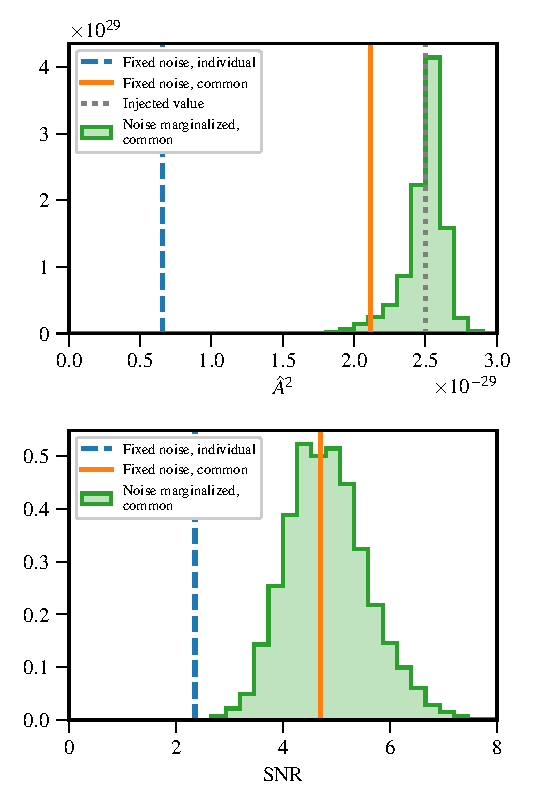
\includegraphics[width=0.95\columnwidth]{plots/optstat_A5e-15_dataset11.pdf}
	\caption{Optimal statistic for a simulated PTA dataset containing an injected GWB. 
			We compare the values found using a fixed-noise analysis 
			with noise parameters taken from 
			individual and common noise analyses 
			(dashed blue lines and solid orange lines, respectively) 
			to the values found by marginalizing over 
			the individual pulsars' red noise parameters (green histograms). 
			The dotted vertical line indicates the injected value, $\Agw^2 = 2.5 \times 10^{-29}$. 
			The fixed-noise analysis 
			using the individual noise results underestimates $\Agw$, 
			while the fixed-noise analysis using the common noise results 
			and the noise-marginalized analysis more accurately recover $\Agw$.}
	\label{fig:os_dataset_sample}
\end{figure}
%\begin{figure}[ht]
%	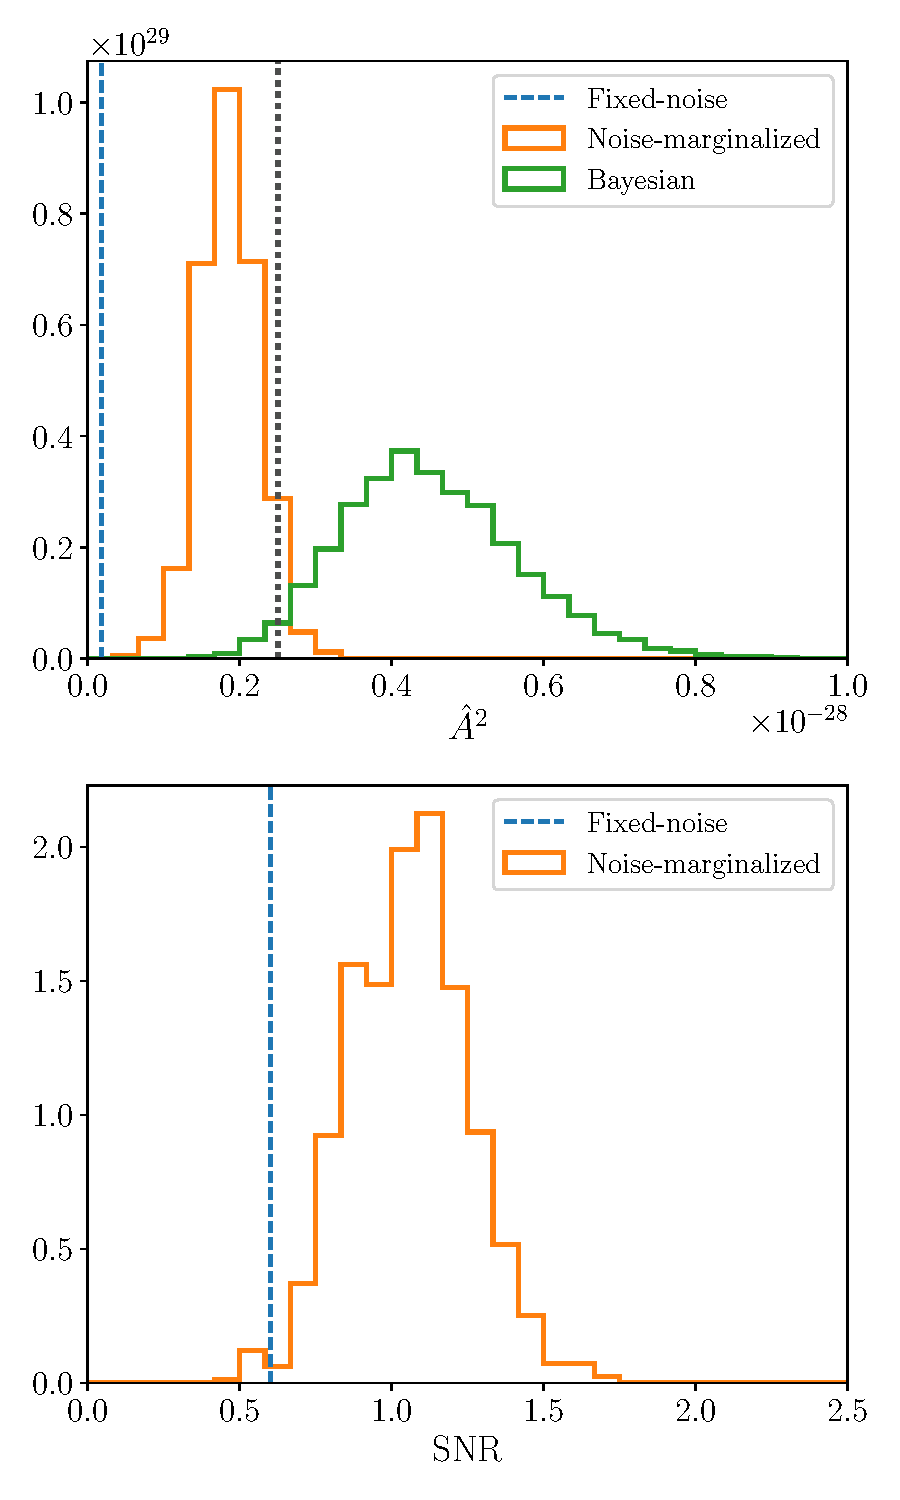
\includegraphics[width=0.9\columnwidth]{plots/os_dataset50.pdf}
%	\caption{Optimal statistic and SNR for a simulated dataset 
%			containing an injected GW background with $\Agw = 5\times10^{-15}$. 
%			We compare the values found using a fixed-noise analysis (dashed blue line) to the 
%			mean optimal statistic and mean SNR found by marginalizing over 
%			the individual pulsars' red noise parameters (solid orange line). 
%			We also include the distribution of $\Agw^2$ found using the results of a Bayesian analysis 
%			for a common red process (solid green line). 
%			The dotted vertical line indicates the injected value, $\hat{A}^2 = 2.5 \times 10^{-29}$. 
%			For this particular realization of the stochastic background, the fixed-noise analysis 
%			gives $\hat{A}^2 = 1.9 \times 10^{-30}$ with $\mathrm{SNR} = 0.60$, 
%			while the noise-marginalized analysis gives $\hat{A}^2 = 1.9\times10^{-29}$ with $\mathrm{SNR} = 1.1$. 
%			For comparison, the Bayesian analysis gives a mean value of $\Agw^2 = 4.5\times10^{-29}$.}
%	\label{fig:os_dataset_sample}
%\end{figure}

In Fig.~\ref{fig:os_datasetstats} we show the optimal statistic 
for 200 different realizations of a GWB with $\Agw = 5\times10^{-15}$ 
computed using the three techniques described above. 
Using the noise values from individual noise analyses 
systematically underestimates the strength of the GWB, 
while using the noise values from a common noise analysis 
more accurately recovers the injected value. 
The fixed-noise analysis using the individual noise results finds 
$\hat{A}^2 = (7.9 \pm 6.8) \times10^{-30}$ and $\rho = 2.3 \pm 1.5$, 
averaging over realizations of the GWB. 
The fixed-noise and noise-marginalized analyses 
using the common noise results both give 
$\hat{A}^2 = (2.4\pm1.2)\times10^{-29}$ and $\rho = 4.1 \pm 1.7$.
\begin{figure}[htb]
	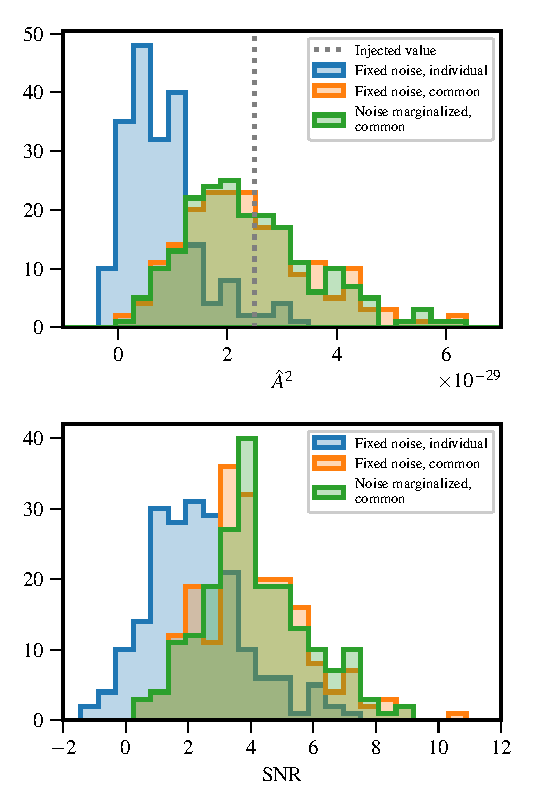
\includegraphics[width=0.95\columnwidth]{plots/optstat_A5e-15.pdf}
	\caption{Optimal statistic and SNR for 200 simulated datasets 
			containing an injected GWB. 
			The dashed vertical line indicates the injected value, $\hat{A}^2 = 2.5 \times 10^{-29}$. 
			We show the values found by fixing the red noise 
			based on the results from individual and common noise analyses 
			(blue and orange lines, respectively) 
			as well as the mean optimal statistic and mean SNR found by marginalizing over 
			the red noise parameters using the results of a common noise analysis (green lines). 
			Using the red noise values from individual noise analyses leads to values of $\hat{A}^2$ 
			that are significantly lower than the injected value, 
			while using the values from a common noise analysis gives values of $\hat{A}^2$ 
			that are closer to the injected value.}
	\label{fig:os_datasetstats}
\end{figure}

The fixed-noise and noise-marginalized analyses give the same results 
for $\Agw = 5\times10^{-15}$, 
but there are differences between them when analyzing datasets 
containing smaller injected values of $\Agw$. 
%Figure~\ref{fig:os_datasetstats2} shows the mean optimal statistic and mean SNR 
%for 100 realizations of a GWB with $\Agw = 10^{-15}$. 
%The fixed-noise analysis using the individual noise values 
%gives a mean value of $\hat{A}^2 = 2.9\times10^{-31}$ and a mean SNR of 1.1. 
%The fixed-noise analysis using the common noise values 
%gives a mean value of $\hat{A}^2 = 8.4\times10^{-31}$ and a mean SNR of 2.1, 
%which the noise-marginalized analysis gives a mean value of 
%$\hat{A}^2 = 1.1\times10^{-30}$ and a mean SNR of 2.4.
%\begin{figure}[t]
%	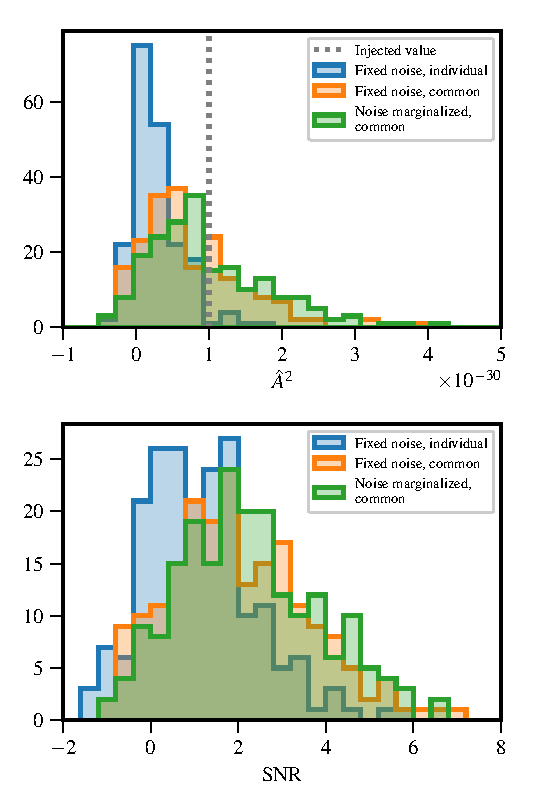
\includegraphics[width=0.95\columnwidth]{plots/optstat_A1e-15.pdf}
%	\caption{Optimal statistic and SNR for 100 simulated datasets 
%			containing an injected GWB with $\hat{A}^2 = 10^{-30}$ (dashed vertical line). 
%			We show the values found by fixing the red noise 
%			based on the results from individual and common noise analyses 
%			(blue and orange lines, respectively) 
%			to the mean optimal statistic and mean SNR found by marginalizing over 
%			the red noise parameters using the results of a common noise analysis (green lines). 
%			Using the red noise values from individual noise analyses leads to values of $\hat{A}^2$ 
%			that are significantly lower than the injected value, 
%			while using the values from a common noise analysis gives values of $\hat{A}^2$ 
%			that are closer to the injected value.}
%	\label{fig:os_datasetstats2}
%\end{figure}
We also compare these three methods 

Figure~\ref{fig:os_compare} shows the distribution of $(\hat{A}^2-\Agw^2)/\sigma$
\begin{figure*}[t]
	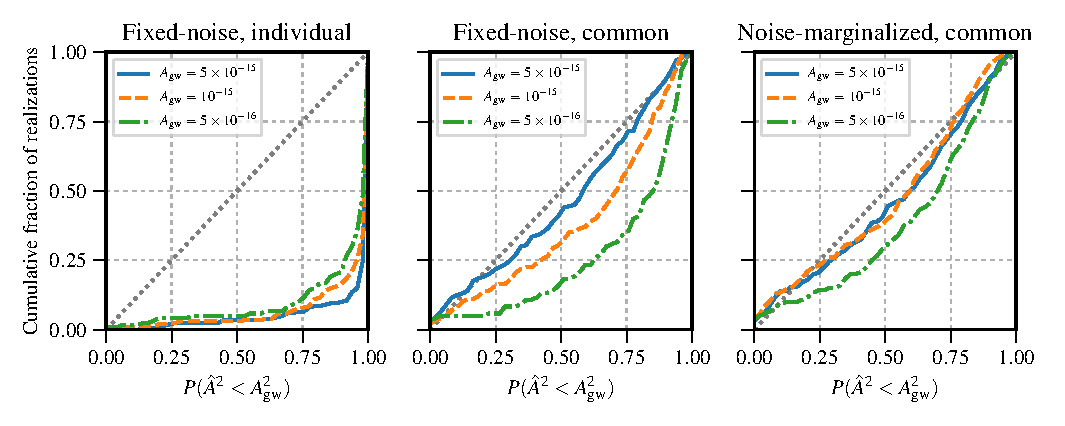
\includegraphics[width=0.95\textwidth]{plots/pp_plot.pdf}
	\caption{P--P plot showing the cumulative fraction of simulations for which $\Agw^2$ lies within 
			a given confidence interval of the measured $\hat{A}^2$. 
			The probability distribution of $\hat{A}^2$ is assumed to be a Gaussian 
			with variance $\sigma^2_{\hat{A}^2}$. 
			The fixed-noise optimal statistic using the individual and common noise results 
			both give biased values of $\hat{A}^2$, particularly for small values of \Agw, 
			while the noise-marginalized optimal statistic gives more accurate values of $\hat{A}^2$ 
			over a large range of injected values of \Agw.}
	\label{fig:os_compare}
\end{figure*}


\section{Monopole and Dipole Spatial Correlations}
\label{sec:spatial}

The optimal statistic is particularly well-suited to compare multiple spatial correlation relations 
because using a different spatial correlation only requires changing the ORF 
in Eq.~\eqref{eq:}. 
\citet{thk+2016} demonstrated how the optimal statistic can be altered to fit for 
multiple spatial correlations at once in order to mitigate common noise sources such as 
clock error and ephemeris error. 
Here we compute the optimal statistic with monopole and dipole spatial correlations 
for the same simulated data sets as in the previous section in order to determine 
how well we can distinguish a GW background from a monopole or dipole signal. 
For a monopole signal, the ORF becomes simply
$\Gamma(\theta_{IJ}) = 1$, 
while for a dipole signal, the ORF becomes
$\Gamma(\theta_{IJ}) = \cos\theta_{IJ}$.

Our ability to distinguish between different spatial correlations 
depends on the strength of the GWB 
and the angular separations between pulsar pairs, $\theta_{IJ}$. 
We can determine the overlap between ORFs corresponding to different spatial correlations 
by computing the ``match statistic'' \citep{cs2016},
\begin{equation}
	\bar{M} = \frac{\sum_{I,J \neq I} \Gamma_{IJ} \Gamma'_{IJ}}{\sqrt{ \left( \sum_{I, J \neq I} \Gamma_{IJ} \Gamma_{IJ} \right) \left( \sum_{I, J \neq I} \Gamma'_{IJ} \Gamma'_{IJ} \right)}} \,,
\end{equation}
where $I$,$J$ index the pulsar number, and $\Gamma$ and $\Gamma'$ are two different ORFs. 
For the 18 pulsars used in these simulations, the 
match statistic for monopole and Hellings-Downs correlations is $\bar{M} = 0.264$, 
and the match statistic for dipole and Hellings-Downs correlations is $\bar{M} = 0.337$. 
These match statistics describe a fundamental limit on our ability 
to identify the spatial correlations of a common red signal as Hellings-Downs 
rather than monopole or dipole 
that depends only on the number of pulsars in our PTA and their sky positions.

Figure~\ref{fig:os_ORF} shows the noise-marginalized 
mean value of $\hat{A}^2$ and the mean SNR 
computed assuming monopole, dipole, and quadrupole spatial correlations 
for 200 simulated data sets. Using a monopole or dipole ORF 
gives a lower value for the mean optimal statistic and mean SNR compared to the 
Hellings-Downs ORF. 
We find a noise-marginalized mean SNR above 1.0 in 97\% of our simulated data sets 
using the quadrupole ORF, and in 50\% and 68\% of our simulated data sets 
using the monopole and dipole ORFs, respectively. 
The mean SNR using the quadrupole ORF, averaged over realizations of the GWB, is 4.1, 
and we find an SNR greater than this using the monopole and dipole ORFs in just 
3\% and 3.5\% of our simulations, respectively.
\begin{figure}[t]
	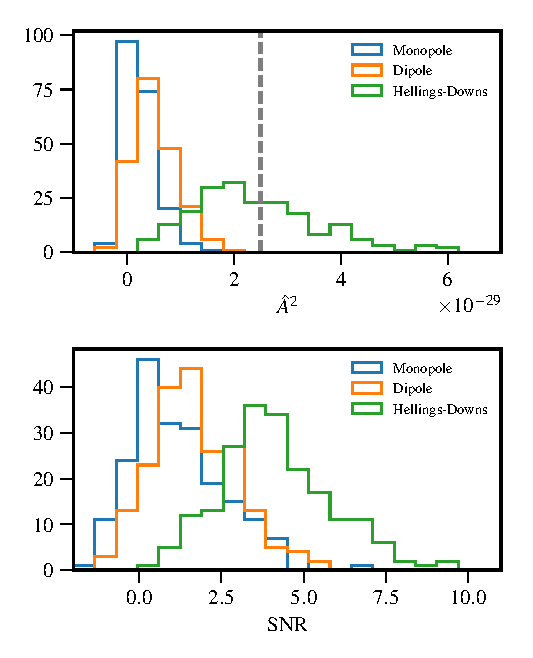
\includegraphics[width=0.95\columnwidth]{plots/optstat_spatial_A5e-15.pdf}
	\caption{Noise-marginalized mean optimal statistic and mean SNR for 200 simulated datasets 
			containing an injected GWB with $\Agw = 5\times10^{-15}$. 
			We compare the values found using monopole (blue), dipole (orange), 
			and quadrupole (green) spatial correlations. 
			The dashed vertical line indicates the injected value, $\hat{A}^2 = 2.5 \times 10^{-29}$.}
	\label{fig:os_ORF}
\end{figure}


\section{Sky Scrambles}
\label{sec:skyscrambles}

Another technique for testing the spatial correlations is through ``sky scrambles,'' 
where the ORF is altered in order to simulate changing the pulsars' positions \citep{cs2016}. 
\citet{tlb+2017} showed how sky scrambles affect the Bayes' factor for simulated data sets. 
Here we perform a similar analysis using frequentist methods.

We used the same scrambled sky positions as were used in \citet{tlb+2017}. 
These positions were chosen so as to minimize the overlap  
between the scrambled ORFs and the true ORF, 
which can be assessed using the ``match statistic'' \citep{cs2016}:
\begin{equation}
	\bar{M} = \frac{\sum_{I,J \neq I} \Gamma_{IJ} \Gamma'_{IJ}}{\sqrt{ \left( \sum_{I, J \neq I} \Gamma_{IJ} \Gamma_{IJ} \right) \left( \sum_{I, J \neq I} \Gamma'_{IJ} \Gamma'_{IJ} \right)}} \,,
\end{equation}
where $I$,$J$ index the pulsar number, and $\Gamma$ and $\Gamma'$ are two different ORFs. 
The 210 sky scrambles used in this paper were generated 
using a particle swarm optimization (PSO) algorithm \citep{ke1995,se1998} 
with the requirement that the scrambled ORFs had $\bar{M} < 0.1$ when compared to the true ORF and to each other.
\sv{Steve, check this section}

Figure~\ref{fig:skyscrambles_dataset_sample} compares the noise-marginalized optimal statistic 
for a particular data set to the distribution of noise-marginalized optimal statistics obtained using sky scrambles. 
For this data set, the noise-marginalized mean optimal statistic is 
$1.9\times10^{-29}$ and the mean SNR is 1.1. 
The distributions of the noise-marginalized optimal statistic and SNR obtained using the scrambled ORFs 
are both centered around zero, 
and for 24 out of the 210 sky scrambles, the SNR is above the true value of $1.1$ ($p=0.11$). 
Figure~\ref{fig:skyscrambles} shows the $p$-values for 210 sky scrambles 
using 425 realizations of the stochastic background. 
For 62\% of simulations the $p$-value is $<0.1$, and for 29\% of simulations the $p$-value is $<0.01$.
%\begin{figure}[htb]
%	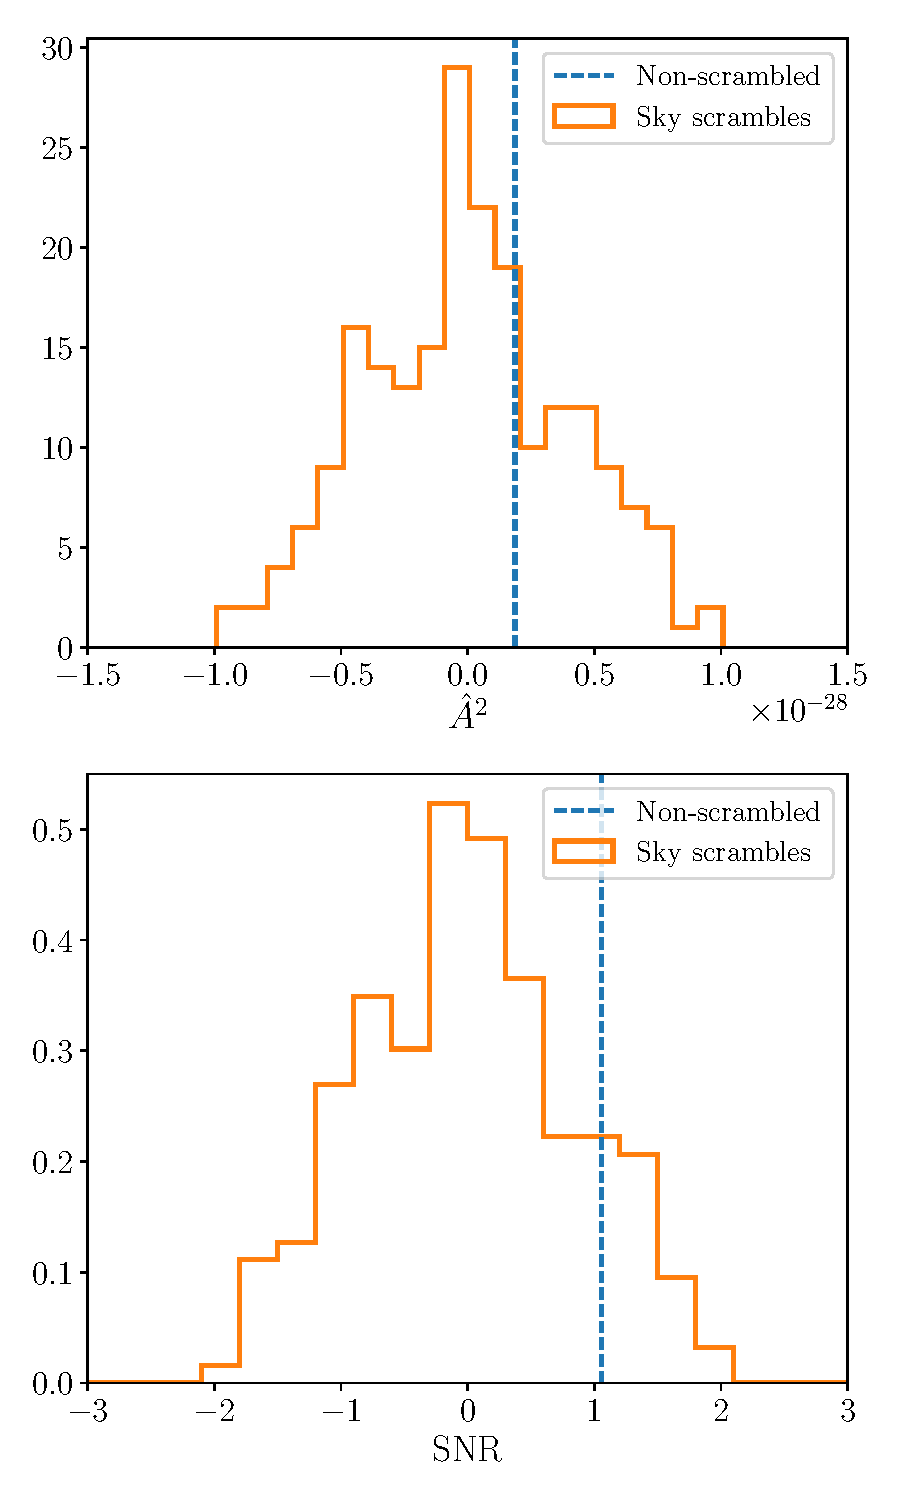
\includegraphics[width=0.9\columnwidth]{plots/skyscrambles_dataset50.pdf}
%	\caption{Comparison between the noise-marginalized mean optimal statistic and mean SNR 
%			with and without sky scrambles for a simulated dataset 
%			containing an injected GW background with $\Agw = 5\times10^{-15}$. 
%			Using the true ORF, we found an SNR of 1.1, while only 24 of the 210 analyses using scrambled ORFs 
%			found an SNR $\geq 1.1$ ($p=0.11$).}
%	\label{fig:skyscrambles_dataset_sample}
%\end{figure}
%\begin{figure}[htb]
%	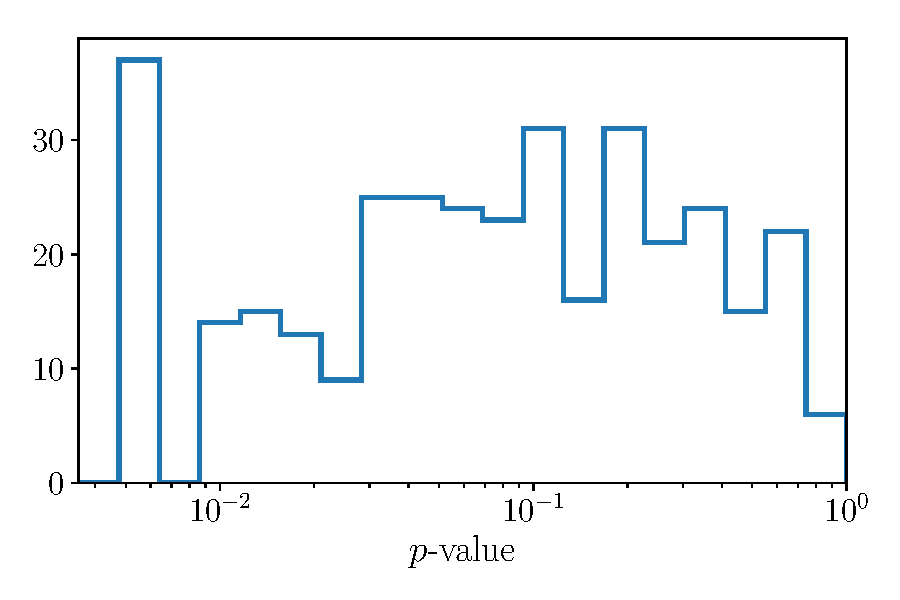
\includegraphics[width=0.9\columnwidth]{plots/os_skyscrambles.pdf}
%	\caption{Distribution of $p$-values for 425 different realizations of the stochastic background. 
%			For each realization, the $p$-value is the fraction of sky scrambled ORFs that gives a 
%			noise-marginalized mean SNR greater than the mean SNR using the correct ORF.}
%	\label{fig:skyscrambles}
%\end{figure}

For five realizations of the stochastic background, we also computed the Bayes' factors for the 
true and sky scrambled ORFs in order to directly compare 
the frequentist and Bayesian detection techniques.
\sv{comparison to Steve's}


\section{Conclusion}
\label{sec:conclusion}

The optimal statistic is a frequentist estimator for the strength of 
an isotropic stochastic GWB in PTA data that searches 
for a common signal with a particular spatial correlation relation 
using a matched filter approach. 
Searching for the spatial correlations characteristic of a GWB 
using a full Bayesian approach is computationally inexpensive, 
whereas the optimal statistic can be computed in a fraction of the time. 
This makes the optimal statistic particularly useful for simulations 
or for analyses where many spatial correlations are compared 
such as sky scramble analyses.

However, the optimal statistic tends to systematically underestimate the strength of a GWB 
when computed for fixed values of the red noise because of 
covariances between red noise in individual pulsars and the GWB. 
In this paper, we introduce an improved method for computing the optimal statistic 
that marginalizes over the individual pulsars' red noises. 
This approach \sv{expand...}


\acknowledgments
We thank Joe Romano and Jeff Hazboun for useful discussions. 
KPI and SJV are supported by NSF Physics Frontier Center Grant 1430284.
JAE was supported by NASA through Einstein Fellowship Grant PF4-150120. 
SRT was supported by appointment to the NASA Postdoctoral Program 
at the Jet Propulsion Laboratory, which is administered by Oak Ridge Associated Universities 
and the Universities Space Research Association through a contract with NASA. 


\bibliographystyle{apsrev}
\bibliography{master}

\end{document}
